\clearpage
\newgeometry{hmargin=2.5cm,vmargin=2cm}

\chapter{Project Contextualization}\label{context}

	\introductionLettrine{T}{his} part gives a first and general glimpse into what was at stake in 
	the realization of the tracking robot. The relevance of the 
	project is justified, the requirements and goals of the project
	are defined, and the global strategy of development is
	presented.

	\section{Project Specification}
	
		\subsection{Motivations}
	
		The main goal of this project was to build a \textit{Deep Learning Tracking Robot}. Many tracking
		robots have been implemented in the previous years, few have used the adaptive, versatile, and 
		now standard robotic Middleware \textit{ROS}\footnote{Which stands for \textit{Robot Operating System}.}.
		In addition, even fewer have ventured combining \textit{ROS} and \textit{Deep Learning} techniques.
		\\\indent Why \textit{ROS} precisely? As defined by Anis Kouba in \cite{ros}, \textit{ROS}
		is an \frstg{} open-source \textit{middleware} \lstg{} that provides a robust and reliable framework 
		to build robots. \textit{ROS} is a voguish tool to create robots with advanced functionalities so much so 
		that it has become the standard to develop robots. \textit{ROS2} is already in part 
		operational. In this project though, 
		it has been decided that the first version of \textit{ROS} will be used since \textit{ROS2} is still 
		in heavy development and \textit{ROS} is better documented than its counterpart. Besides, 
		some sensors used in this project, such as
		the \textit{ZED camera}\footnote{See \vref{hardwareoverview}.},
		have packages that are still in beta version, hence less reliable than the ones
		of \textit{ROS}.
		\\\indent Why is \textit{Deep Learning} suitable for robotic applications? In general, \textit{AI}
		\footnote{Artificial Intelligence, which comprises \textit{Deep Learning}.}
		is really adapted for critical algorithms, such as embedded codes
		on robots, since the performances are much higher than with traditional implementations. By traditional
		implementations, one could for instance consider iterative algorithms where for a particular task 
		all processes are hand-implemented. The conventional solution 
		that comes to mind regarding tracking is an \textit{RGB} tracking, that is to say an 
		algorithm that tracks the color in a frame\footnote{image.} by applying 
		color filters. \textit{AI} enables much finer and more robust
		implementations since the \textit{model},
		which can be regarded as the applied processes, can evolve by itself through diverse methods such as training.
		 
		\subsection{Requirements}
		
		In order to realize the tracking robot, several requirements had to be met in this
		project. First of all, the robot had to reuse an old \textit{Race Car} platform comprising
		the chassis, the wheels \dots all the mechanics. The platform is the \textit{H1 model}
		of the \textit{monster Car} \cite{datasheet}.
		The brain of the robot, that is to say 
		the embedded computer had to be the \textit{Jetson Nano} designed by \textit{Nvidia} \cite{nano}. By and
		large, to build the tracker the material of the laboratory had to be used as much as 
		possible, and the equipment bought had to remain affordable.
		%TODO image of the old platform rc car
		%TODO image of the jetson nano
	
	\section{Strategy}
	
		\subsection{Different periods}

		Developing a robot is a critical task, and has to be conducted thoroughly. 
		In this regard, \textit{ROS} builds a framework for developing 
		robots in a more organized way. For each task to implement, 
		the work-flow has always been the following: research, simulation, isolated 
		tests, integration.
		\\\indent Before even implementing something and integrating it, one should 
		research all the possibilities that are offered to them. Then one of the 
		easier or maybe most sustainable options could be chosen. Yet, even the
		tests, simulation, and integration has to be thought and foreseen beforehand.
		\\\indent Simulating robots, without depending on the hardware is
		a needed step.	 A specific hardware has always some specificities that
		could hide some issues and unpredictable behaviors. As a matter of fact, 
		simulating algorithms that will be integrated in the robot afterward in 
		a controlled environment prevents any hardware based issue to shadow
		our understanding of the basic implementation of
		the \textit{software}.
		\\\indent Once the simulation is in place, it is then 
		recommended to test the simulation as much as possible in order
		to unveil some detrimental singularities. In the case of the hardware, 
		each component has to be tested independently before integration
		\footnote{Especially, some driver issues are sometimes really 
		hard to pinpoint.}.
		\\\indent The final step is to integrate the work in the robot, and
		to test it to see if the robot behaves as expected or if there 
		is any regression.
		\\\indent A robot is not just a piece of software, it is a system 
		where the interaction of the software and the hardware is by 
		definition the future behavior of the robot.
		
		\subsection{Different aspects}

		The development of a robot encapsulates different areas or type of work.
		In the construction of the tracker, principally two aspects 
		have been tackled, the hardware, and the software.
		\\\indent In the first place, the hardware has to be well-chosen beforehand.
		The motor had to replaced, the \textit{wifi} access had to be added, batteries 
		had to be chosen \dots to fit the requirements of the tracking robot.
		\\\indent In the second place, the sofware has to be implemented. Precisely, 
		the tracking algorithm had to be chosen, and the \textit{ROS} architecture had 
		to be designed.
		\\\indent For the entire project, the philosophy was to try to have 
		a working first prototype as soon as possible. In a nutshell, 
		having a hardware and software which are compatible, and then refining
		the existing platform. Indeed, \textit{ROS} provides here another
		crucial boon, for it enables us to have an evolutive architecture 
		where each part can be replaced easily without 
		undermining the overhaul process. For instance, once 
		an architecture is working, the tracking technique could
		be easily replaced.
		\\\indent Throughout this report, which presents the 
		results of the project, three questions will be answered:
		\begin{itemize}
			\item[\textbullet] How was the hardware selected?
			You can find the answers to 
			this question in the part \vref{hardware}.
			\item[\textbullet] How was the tracking algorithm implemented? Which belongs 
			more to the software. You can find the answers to 
			this question in the section \vref{tracking}.
			\item[\textbullet] How was the \textit{ROS} architecture designed? 
			Which belongs more to the software. You can find the answers to 
			this question in the section \vref{ros}.
		\end{itemize}
		
\chapter{State of the art}\label{stateofart}

		\introductionLettrine{I}{n} order to build the tracker, the first step was to choose the
		hardware of the robot. Secondly, the \textit{ROS} architecture had to be decided
		and thirdly the tracking algorithm had to be implemented. This part 
		presents a brief overview of different existing projects and solutions 
		that could have been selected throughout the project. All the projects
		presented and listed here will then be compared and the choices
		made will be underpinned in the parts \vref{hardware} and \vref{software}.
		
		\section{Building an electric car}\label{buildingcar}
		
		Several projects have aimed to realize an electric car robot, sometimes autonomous. 
		Having in mind these projects can give some piece of advice on how it is common 
		to design such systems.
		\\\indent Some projects have used the on-board computer \textit{Jetson Nano}. 
		One can name the following robots : \textit{Jetbot} \cite{jetbot}, \textit{Kaya} \cite{kaya}.
		These robots are both designed by \textit{Nvidia}, the designers of the 
		\textit{Jetson} board series\footnote{Jetson Nano, Xavier, TX1, TX2 \dots}. It 
		is notably interesting to take as example their hardware selection since they
		use the same embedded computer the tracker use.
		\\\indent Other \textit{RC-cars}\footnote{\textit{Remote Control Car}.} use other types of embedded computers.
		However, the hardware architecture with regard to \textit{RC-cars} is 
		almost always the same. With either the \textit{DeepRacer} of \textit{Amazon} \cite{deepracer}, or
		the \textit{Pi-Car} \textit{raspberry} powered car \cite{rasp}, or 
		\textit{Ghost} car \cite{ghost}, or the \textit{Roscar} \cite{roscar}, or
		the \textit{F1tenth} car \cite{f1tenth}, or the \textit{Donkey} car \cite{donkey}, the architecture
		follows some fundamental principles.
		\\\indent The selection of the hardware is discussed further in the part \vref{hardware}.
		
		\section{Tracking}\label{statearttracking}
		
		Multiple ways of tracking a target exist \cite{learnopencvtracking}, in this project the most
		common one was used : a \textit{visual tracking}. Visual tracking
		is basically based on the processing of images or frames taken by a camera. 
		\\\indent More precisely, the mission of the tracker implemented
		in this project is to follow
		a specific object in a frame
		\footnote{Given by a camera for instance.}, to be able to 
		learn the object in that process, and even to be able to recover the target after 
		any occlusion. Looking at the deep learning models and algorithms 
		which have been developed in the recent years,
		some could be more labeled as detection algorithms, do not really learn the specificities 
		of the target, and even track multiple targets. For instance, the network \textit{Yolo} 
		\cite{bjelonicYolo2018} is rather designed for multi-tracking and 		not to follow a specific target. 
		\\\indent Considering deep learning models that are able to 
		track a specific target the database \textit{GOT-10k} has produced
		an enumeration and ranking of the current most effective techniques \cite{trakinglist}.
		\\\indent For sure, in order to automate the robot, a detection algorithm
		could precede the tracking.
		 
		
		\section{Using ROS}
		
		Developing with \textit{ROS} gives also an incredible
		advantage to any roboticist. In fact, some \textit{ROS packages}
		which are totally open-source already provide cutting-edge algorithms
		such as sensor fusion by Kalman filtering, \textit{SLAM}
		\footnote{Simultaneous Localization And Mapping.}. Unfortunately, 
		applied to specific object tracking few \textit{ROS} packages were developed, and
		the existing ones do not use deep learning techniques at all.
		\\\indent Nevertheless, some \textit{ROS interfaces} were implemented
		for \textit{ROS}, which can allow one to use a tracking algorithm
		compatible with the \textit{ROS interface}, also often named
		\textit{bridge} \cite{mtf}. The main problem is mainly that the implemented
		programs are not up-to-date which renders the integration
		in \textit{ROS} sometimes almost impossible due to software dependencies.
		\\\indent Apart from that, several projects, almost all shared on
		\textit{github}, implement tracking solutions. However, they 
		either do not use deep learning, or are not supported by \textit{ROS} 
		anymore. The book \textit{ROS Robotics Projects} presents
		a well-documented tracking project, though no
		deep learning techniques are used \cite{rosprojects}. Yet, 
		the \textit{ROS} architecture inspired some of the realization 
		of the own architecture of this project.
		\\\indent A paper tackled a robot for person following \cite{personfollowing}.
		Yet, the tracker in this project is not just intended to track a person, 
		but more generally any object.

%%%%%%%%%%%%%%%%%%%%%%%%%%%%%%%%%%%%%%%%%%%%%%%%%%%%%%%%%%%%%%%%%%%%%%%%%%%%%%%%%%%%%%%%%%%%%%		

\chapter{Hardware}\label{hardware}

\introductionLettrine{F}{irst} of all, before even thinking about the tracking process, and
the behavior of the robot, the existing platform had to be fixed, and if needed adapted
to the current needs of the project. This part starts by presenting the latest architecture 
of the tracking robot, an then breaks this architecture apart by giving an overview of
each challenge which had to be tackled.
	
	\section{Hardware architecture}
		
		\subsection{Overview}\label{hardwareoverview}
		
		It is crucial to chose wisely the hardware of the robot in the first place, since
		the software could be seen then as an exploitation of the hardware of 
		the robot. The initial hardware of the robot did comprise
		a servomotor, a \textit{brushed DC motor}\footnote{More is explained 
		on that in the section \vref{motor}.}, and a motor controller, or \textit{ESC}, which
		stands for \textit{ Electronic Speed Controller}.
		\\\indent This initial architecture had to be adapted for several reasons.
		The latest hardware architecture of the tracking robot is
		presented on figure \vref{hardwarearchitecture}, which
		shows each component and how each interacts with each other.
		\\\indent Let's explain a bit what are the crucial parts
		that constitute a tracking robot. The target tracking process used
		in this project is based on image and depth inputs, but to be more
		precise, on a \textit{stereo camera}. A \textit{stereo camera}
		provides basically two types of information : depth and color.
		For this purpose the \textit{ZED camera} of \textit{Stereolabs}
		was used \cite{zeddoc}. The processing of the frames
		given by the camera is done on the embedded computer
		\textit{Jetson Nano}. Regarding the actuators, a servomotor
		controls the bearing of the car, and a motor controls the speed
		of the car through an \textit{ESC}. In order to communicate
		with the motor controller, or \textit{ESC} a \textit{PWM shield}
		was needed. Basically, a \textit{PWM} signal, which stands for
		\textit{Pulse Width Modulation} in this case, is a certain type
		of signal which are characterized by their duty cycle. This 
		fundamental parameter is equivalent to the command sent 
		to the \textit{ESC}. At this end, the \textit{PWM shield} PCA9685
		of Adafruit was used \cite{adafruitpwm}. Ultimately, since
		in the field of mobile robotics, robots tend to be mobile by definition,
		the tracking robot had to be powered on its own. To 
		meet that constraint two batteries were added. From all that has
		been mentioned in this paragraph, only the initial servomotor was
		saved.
		
		\FloatBarrier

		\begin{figure}[!htbp]
			\centering
			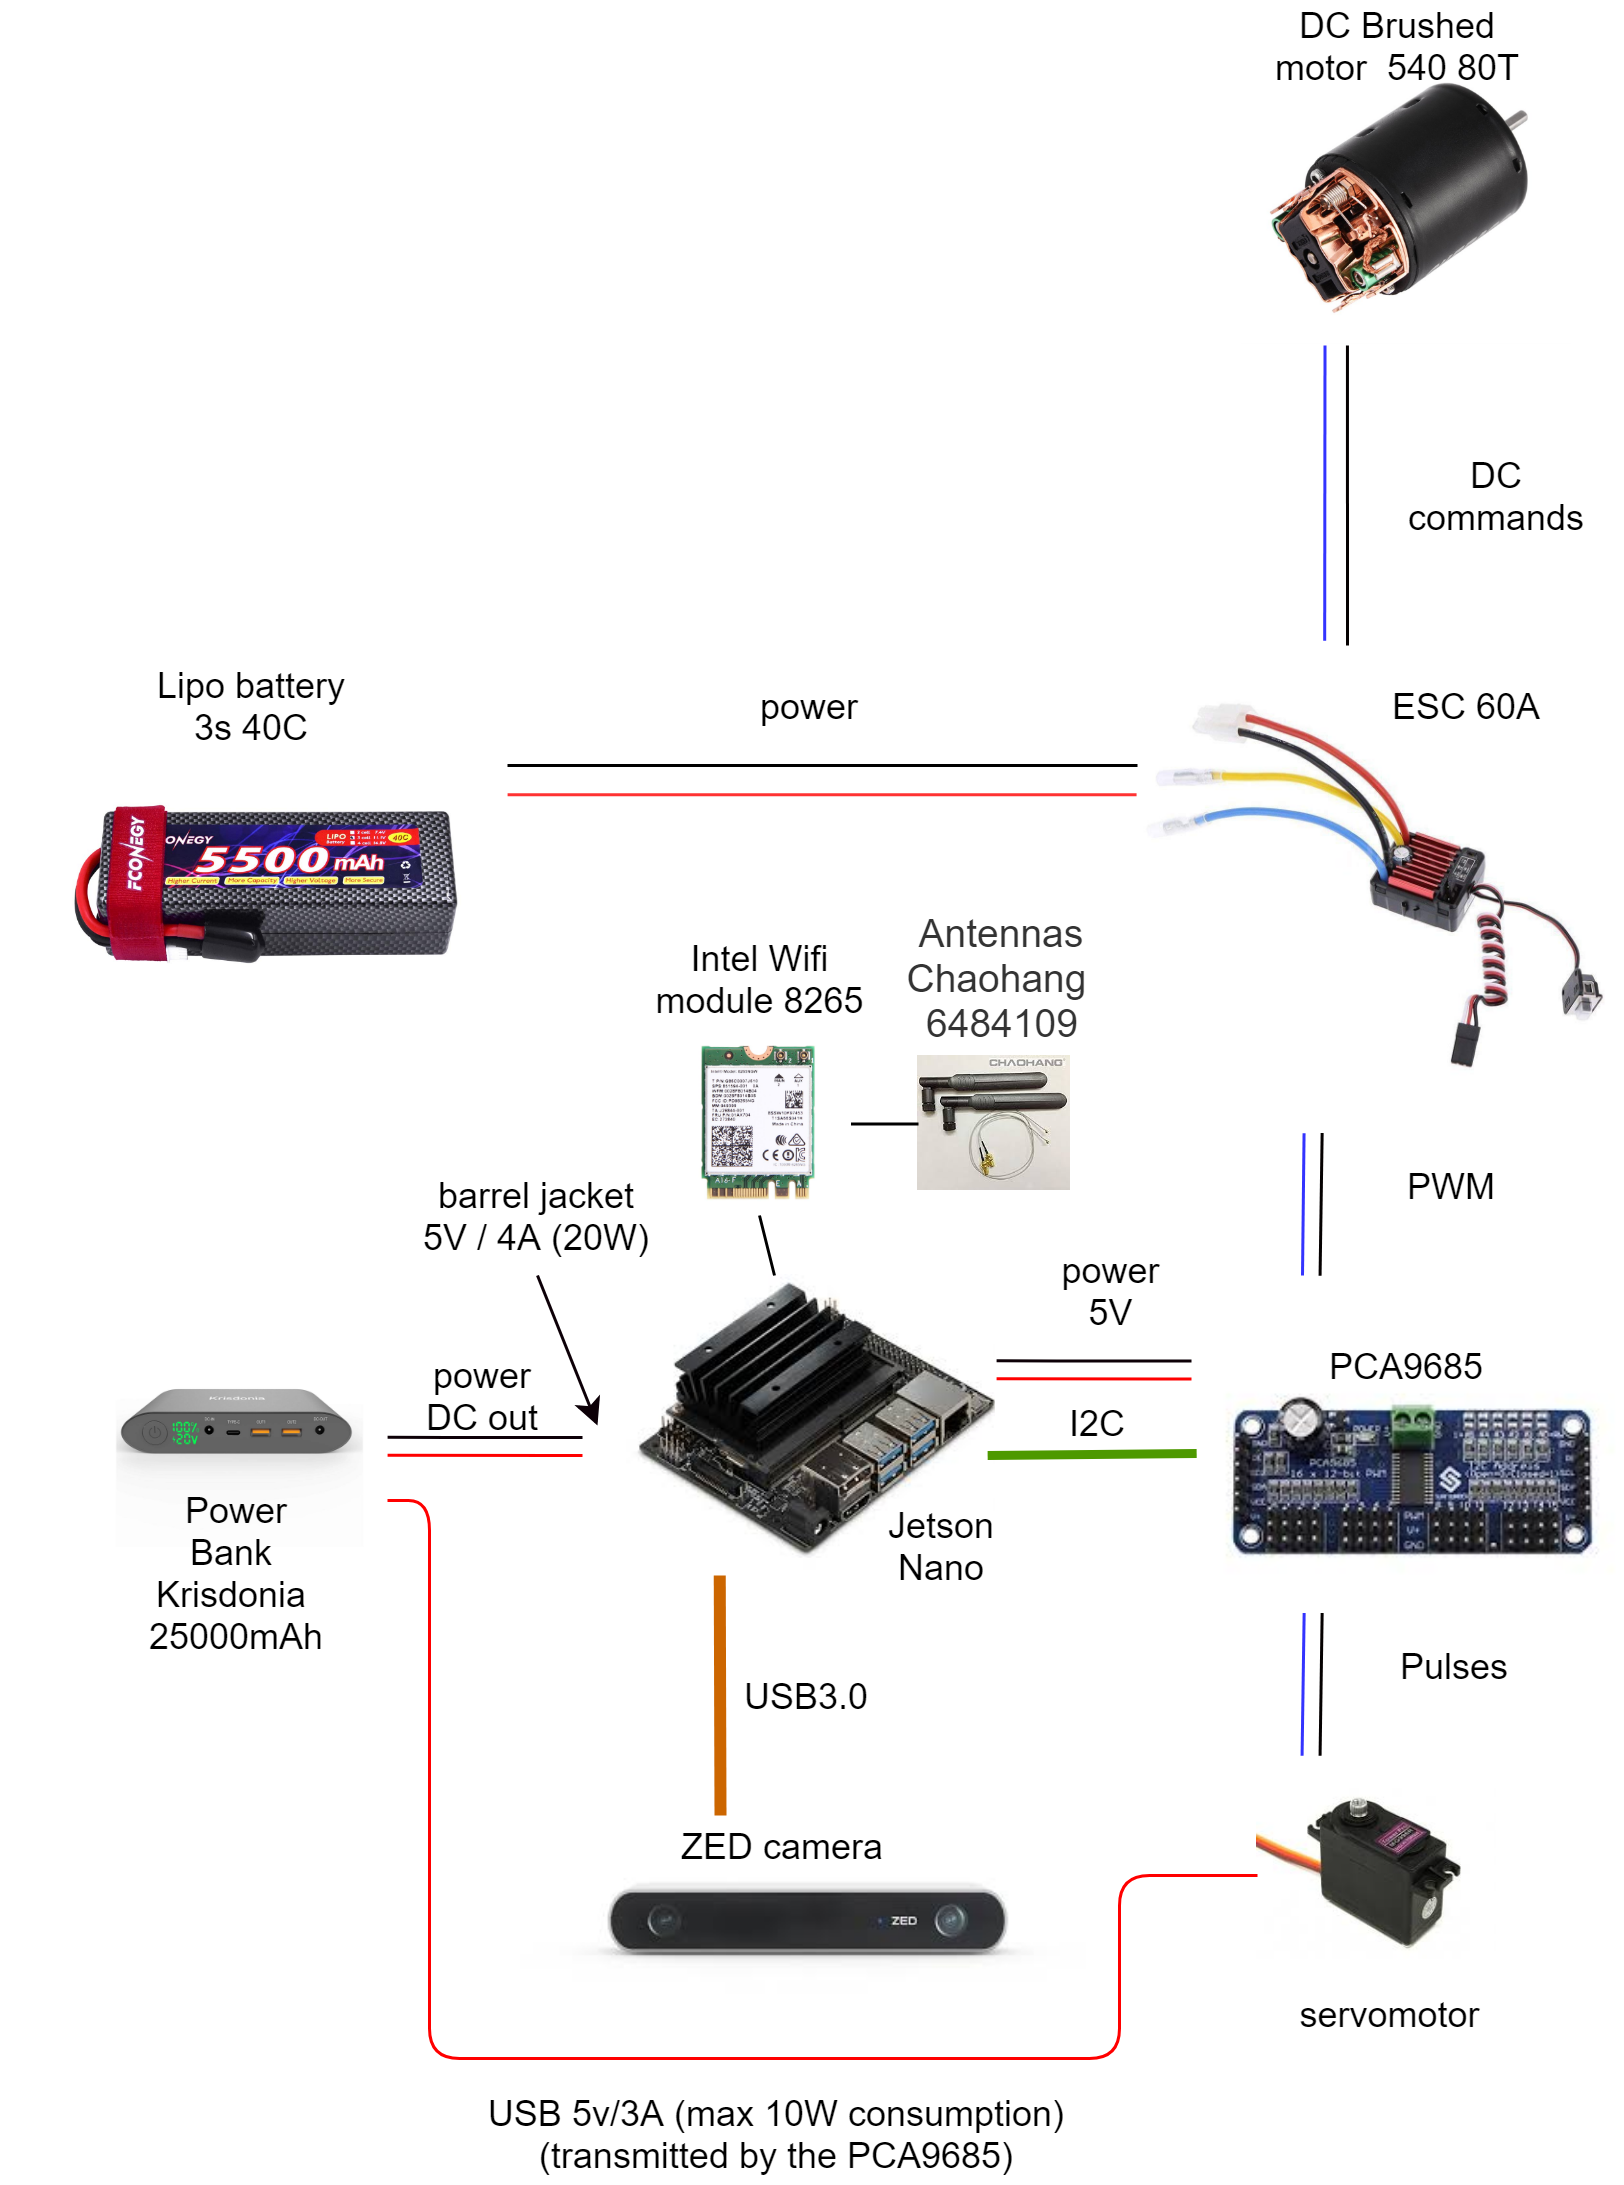
\includegraphics[width=1.0\columnwidth, height = 1.3\columnwidth]{imgs/hardware.png}
			\caption{Hardware architecture.}
			\label{hardwarepng}
		\end{figure}

		\FloatBarrier

		\subsection{Components list}
		
	\section{Low speed control}\label{motor}
	
		\subsection{Motor}
		
		After having fixed the existing \textit{RC car}, the speed was unfortunately 
		too high to meet the likely processing speed of the embedded computer.
		The next step
		was then to find a way to slow down the robot. 
		\\\indent The first constraint was to avoid changing the mechanics as much as
		possible. Changing the gear box, without buying a new \textit{ESC} and a new
		motor could have been possible. Yet, it would have required to alter 
		the entire mechanics of the \textit{RC car} platform. Thus, this option was 
		not considered.
		\\\indent How is it possible then not to modify the mechanics and
		at the same time to decrease the speed? If the mechanics was to 
		be kept identical, that is to say that the power chain should 
		remain untouched, the motor has to remain of the same dimensions.
		This is why as new motor, a \textit{brushed DC motor} was in part 
		chosen. Economically talking, a \textit{brushed} motor is far cheaper
		in comparison to its counterpart the \textit{brushless} motor. Yet, the
		speed has still not been decreased.
		\\\indent To understand how it is actually possible to 
		slow down a \textit{DC motor} it is essential to fathom the 
		existing relation between the torque applied to the charge
		and the \textit{RPM}\footnote{Revolutions Per Minutes.},
		or in other words the angular speed 
		of the shaft of the motor. Basically, the angular speed is
		inversely proportional 
		to the torque. Thus, in order to decrease the angular speed, a 
		\textit{brushed DC motor} with more torque had to be chosen. \cite{bonanza, motor}
		
		\subsection{Motor Controller}
		
		A \textit{DC motor} without a controller is not very useful. At this 
		stage, a controller had to be selected in order to set by commands
		the angular speed of the motor.
		Numerous strategies exist to regulate the speed of a \textit{DC motor}.
		For instance, it is possible to use specific motor controllers \cite{f1tenth}, 
		transistors, or \textit{ESCs}. From all the projects introduced
		in the state or the art part \vref{buildingcar}, a majority 
		uses \textit{ESCs}.
		\\\indent Yet, the race car of the \textit{MIT}\footnote{Massachusetts Institute
		of Technology, USA.} employs \textit{VESC}, which stands for \textit{Vedder 
		Electronic Speed Controller} \cite{mitracecar}. Such \textit{ESCs} were designed
		to provide more flexibility in the control of the low speeds. However, their price
		were far too high to be considered in this project.
		\\\indent All in all, a new brushed motor \textit{ESC} was bought.
		\\\indent \textit{ESCs} were first designed for \textit{RC cars}, that is to say for 
		remote control in general. This is why, the commands that should be given to them
		as inputs are signals transmitted by remote controller, \textit{PWM signals}. In order
		to generate such signals the \textit{GPIO}\footnote{Which stands for \textit{General Purpose Inputs Outputs}.}
		pins or outputs of the \textit{Jetson Nano} 
		provide some relevant functionalities. The jetson nano has two channels that
		can generate \textit{PWM} signals. Yet, the \textit{PWM shield}  PCA9685
		of Adafruit is more reliable, since its function is exclusively to generate
		such signals. The selected solution was to use the \textit{GPIO} pins 
		to generate \textit{I2C}\footnote{Two-wire communication 
		protocol that allows to address several devices or give several 
		orders at the same time to external devices from a microcontroller.} signals to communicate
		with the \textit{PWM shield}. The \textit{PWM shield}
		then outputs the right \textit{PWM signals}.\cite{tk1servo,nanogpio,nanogpiolayout} 
	
	\section{Power consumption}
		
		\subsection{How many?}
		% How many batteries?
		The first question that should came to mind is not which type of battery
		should be bought, or even
		how much power the hardware requires, but how many batteries the robot 
		needs. It is common in robotic applications and more 
		extensively in any system to split the power supply into two parts.\cite{racecarj} 
		\\\indent Actuators, that is to say for instance motors
		or servomotors, tend to require far more power than the embedded computer. Besides, 
		should the actuators draw too much current\footnote{It often happens that the 
		actuators may induce current peaks.}, the embedded computer will switch off. Thus, 
		as a matter of safety, it is crucial to isolate the power source of the actuators
		from the one of the embedded computer. This explains the choice of two separate 
		batteries.
		% split the power source in more than two parts : usb hub --> battery for the computer + for the actuators : minimum.
		\\\indent By and large, the takeway is that the embedded computer must not, 
		in any circumstances, be switched off, since the hardware will still 
		apply the last commands stored in the more detrimental cases. It is 
		also highly recommended to use a self-powered \textit{USB-Hub}
		to plug any subsequent device to the embedded computer, which 
		may draw too much current from the embedded computer \cite{racecarj}.
		That advice was not applied in this project, and could be
		seen as a point of improvement.
		\\\indent All these choices were further underpinned by 
		the projects presented in \vref{buildingcar}.
		
		\subsection{Which ones?}
		% Battery for the ESC and motor : actuator.
		On the one hand, regarding the motor, which is the actuator that 
		draws the more power among the hardware of the robot, an independent 
		\textit{Li-Po} battery has been chosen. This choice
		was further promoted, for \textit{Li-Po} batteries, in 
		comparison to \textit{NiMH} and \textit{Ni-Cd} batteries, 
		tend to be more efficient and start to gradually 
		supersede them.
		% How do we power the computer, and the motor? Pb when powered via micro-usb ---> powered via barrel jacket :
		% battery for the servomotor
		\\\indent On the other hand, regarding the power source of the embedded computer, with 
		the normal power input through \textit{micro-usb} the power supplied
		was maximum 10 Watts, and the jetson nano used to be turned off. As a matter of fact,
		after some tests, it appears that it was due to an under-powering of the 
		\textit{Jetson Nano}, although the \textit{Jetson Nano} was not connected
		to any other device. Multiple ways exist to power the \textit{Jetson Nano}.
		Powering the board through the \textit{Power Jack}, which gives maximum 20 Watts, 
		was the chosen solution. Hence, the battery \textit{Krisdonia 25000mAh} was bought to meet that 
		requirement \cite{nanopowerbank}. In addition, it enables to plug more external devices to the \textit{Jetson Nano}
		and fasten its overall performances.
		\\\indent The servomotor is still not powered. Servomotors are commanded
		via \textit{PWM signals}. Those ones are generated with the \textit{PWM shield}, also 
		used for the communication with the \textit{ESC}. The \textit{PWM shield} needs to power the 
		servomotor though. This is done by using the \textit{V+} external power input of
		the \textit{Adafruit shield}. Since the \textit{Krisdonia 25000mAh} is powerfull 
		enough with a \textit{DC ouput} for the\textit{Jetson Nano} and two other independent
		\textit{USB power outputs} with a $5V/3A$, the servomotor is powered through the \textit{PWM shield}
		with the \textit{Krisdonia 25000mAh} battery.
		% Present the battery adviced by jetson hacks.
		% How many power do our hardware need?
		\cite{jetsonhacksmorepower,nanoguide,elinuxdoc}
		
	\section{Remote control and processing}
		
		% Remote control of the robot, supervising, displaying information
		% other interest : using more powerful GPUs for deep learning applications : processing the frames on 
		% a remote computer.
		When the tracking robot is in mission, it is essential that 
		at each time the information gathered and processed by the
		robot can be displayed and monitored by a human agent.
		For instance, it is useful to store the data on a remote 
		computer, to display some curves, or 
		simply to command the robot remotely when the tracker encounters
		some hurdles. Communication can be established via \textit{SSH}\footnote{Secure Shell.}
		in a terminal environment. Yet, the robot needs to be able 
		to be connected to a network, and unfortunately, the 
		\textit{Jetson Nano} does not provide any way to do that. The most common way 
		to achieve that is by using a \textit{WiFi Module}. A huge 
		variety of such devices can be find on the market, the question 
		is then which one of those is the most suitable for the 
		targeted application.
		\\\indent Another aspect of the decision should take into 
		account that it would be more efficient and sustainable 
		to be able to process the frames of the camera on
		a remote computer more powerful than the \textit{Jetston Nano}.
		However, to send frames via \textit{WiFi} the \textit{ WiFi Module}
		must possess a relevant bandwidth and a faster than average communication
		speed. For this reason the module \textit{8265NGW} of Intel was chosen, which 
		delivers up to 867Mbps \cite{wifi}.
		
	\section{Performances of the embedded computer}
	
		The performances of the embedded computer are crucial in 
		any robotic application.
		At first the \textit{Jetson Nano} was too slow 
		to do anything else than acquiring the image of the \textit{ZED camera}.
		In order to increase those performances a bigger \textit{SD card} of 
		about 64 GB had to be added.
		\\\indent Improving the processing speed of the \textit{Jetson Nano}
		could also be done by artificially increasing the \textit{RAM}\footnote{Random Access
		Memory.} of the board, which comes with a limited 4 GB of \textit{RAM}. The latter
		was not put in place, it is highly recommended in the future though. \cite{swap}
	
	\section{Unit Tests}

		Before trying to integrate anything, that is to say 
		to use the hardware inside a \textit{ROS} framework 
		or to merge hardware and tracking, the hardware was
		tested independently.
		\\\indent Especially, regarding the actuators, 
		being the servomotor and motor, a low-level library 
		was written in python, \textit{hardware.py}, which is
		presented in the appendix \vref{hardwarelib}. 
		It belongs to the software of course, but since the low-level 
		library is aimed to directly drive the hardware, this 
		section can be considered inside the hardware part. 
		\\\indent In fact, this library enables to create
		a \textit{python object} for each piece
		of hardware. Each object provides
		some high level methods, which can 
		then be used in a more complex \textit{ROS}
		architecture. Parameters were also set 
		in order to transfer a low-level command
		to a high-level command. As expected, 
		the speed was sufficiently decreased for
		the tracking application.
		

\chapter{Software}\label{software}

	\introductionLettrine{T}{he} hardware selection has been discussed in the part \vref{hardware}. 
	Once the hardware architecture is defined and tested, the software 
	part must be implemented in order to merge them together. The software
	comprises mainly two challenges : the realization of the tracking and the
	conception of the \textit{ROS} architecture.
	
	\section{Tracking}\label{tracking}
	
		% NOTES
		% strategy of development, position of the problem
			% pretrained model
			% then complicate it
		% Why GOTURN? opencv, easy of use first, and then maybe my own, can be trained
			% add the goturn paper
		% ROS interfacing and GOTURN
		% Unit Tests : really good for human faces (it was apparently more trained on human faces), 10-30FPS with 
		% the webcam of the computer, a static image
		
		\subsection{Overview}
		
		As explained in \vref{hardwareoverview} and \vref{statearttracking}, in this project
		the tracking algorithm is implemented with a deep neural network and takes as input
		the color frames of the \textit{ZED camera}. The goal is
		to have a tracking algorithm able to follow a specific target in 
		a sequence of frames.
		\\\indent The approach to the problem was to find a tracking algorithm or model 
		which is pretrained. Basically, starting with the easiest solution and 
		then, if needed, refining it. Another idea was also to 
		have the model running in a controlled environment and then, once tested, 
		interfacing it with \textit{ROS}.
		
		\subsection{Goturn}
		
		Among the numerous and variegated tracking solutions presented in 
		\cite{trakinglist} the pretrained model \textit{GOTURN} was chosen.
		\\\indent First of all, only the tracking algorithms that were
		implemented in \textit{python} were selected for compatibilities issues.
		\textit{GOTURN} was also the best choice regarding the ease of 
		programming. It is implemented inside the \textit{OpenCV}
		library, which is one of the most widely used
		computer-vision library worldwide, and which renders it far easier
		to integrate the tracking model in the \textit{ROS} architecture
		afterward. \cite{goturn}
		\\\indent \textit{GOTURN} is also sustainable and flexible, for it is
		possible to acquire the untrained model for a more 
		specific application.\cite{goturnpy}
		
		\subsection{ROS interface}
		
		Making the \textit{GOTURN} tracker work inside
		the \textit{ROS} framework was not that easy, 
		although it was easier than the other available solutions.
		% python environment for opencv, docker
		Running the \textit{GOTURN} function provided 
		in the \textit{OpenCV} library needed 
		to have a version of \textit{OpenCV} higher than $3.4.2$ \cite{learnopencvgoturn}.
		However, since
		\textit{ROS} relies on \textit{Python 2.7}, 
		it only comes with an older version. I was not
		able to uninstall this library since it was
		a dependency for other \textit{ROS} packages. The 
		workaround was to create a \textit{Python Environment}
		using \textit{virtualenv} on \textit{Ubuntu}, and then 
		to specify this \textit{Python} interpreter of this
		particular environment in the code of the tracker
		using the \textit{shebang}, the first line of code
		where the interpreter is specified.
		% ROS interface, image message
		\\\indent Once the right version of
		\textit{OpenCV} was installed, and the \textit{Python}
		interpreter suitably indicated, the \textit{GOTURN} function
		needed to be interfaced with the \textit{ROS} environment.
		\textit{ROS} uses its own type of data, named \textit{messages}.
		For instance an image or frame is an \textit{Image.msg} message \cite{imagemsg},
		which totally differs from the way \textit{OpenCV}
		represents images.
		The bone of contention here was to be able to 
		convert the \textit{ROS} datatype into the \textit{OpenCV} one.
		This is called \textit{Interfacing}.
		Fortunately, the package \textit{cv\_bridge} provides that 
		functionality \cite{rosdoccvbridge}. 
		\\\indent For sending frames between two devices connected
		to the same network the \textit{ROS} package \textit{image\_transport}
		can be used \cite{rosdoctransport}. The \textit{ZED camera} already
		provides compressed image channels, using the \textit{image\_transport} package.
		\\\indent The code was then adapted to satisfy \textit{ROS}
		functionalities. 

		\subsection{Unit Tests}
		
		The tracking algorithm was first tested outside the \textit{ROS}
		framework. Actually, the frame rate was around 50 \textit{FPS}\footnote{Frames per second.},
		half of what was advertised
		in the original paper \cite{goturn}. Yet, this may be due to
		the \textit{OpenCV} implementation, which is not 
		the initial one, though inspired of it. 
		These performances seem to suffice for the realization of the tracker though.
		\\\indent The next step was to interface this implementation 
		with \textit{ROS}. The tests comprised a static image, and 
		the webcam of the computer. The performances were unchanged.
		\\\indent These tests also demonstrated that the \textit{OpenCV}
		\textit{GOTURN} model was really accurate at tracking
		humans. Yet, when it came to everything else, the model 
		was lost easily. The assumption here may be that 
		the model had been more trained on human targets. 
		Regarding the reliability of the tracking given 
		the nature of the target, the performances
		could be increased by retraining the model \cite{goturnpy}.
		
	\section{ROS}\label{ros}
	
		\begin{comment}
		
		The Bascis of ROS : add some ROS books
			master
			topic 
			nodes
			services
		Overview of the ROS architecture
			Position of the problem
			How does the ROS architecture work? Function of each node
			Two version of the ROS architecture
				remote processing
				local processing
			present the state equation for the variables of the controller
		Speed regulation
			PID controller
		Bearing regulation
			PID controller
		Unit tests without the hardware : everything was simulated
			test on one computer : simulation = without the hardware
			x test with the remote computer : still without the zed camera and actuators
				
		\end{comment}
		
		
		 % TODO
		\subsection{ROS Basics}
		
			\textit{ROS} is a robotic \textit{middleware}. Basically, it
			handles the interactions between the processes
			running on a robot.
			\\\indent In the \textit{ROS} world, a process, for 
			instance a program which sends commands to a motor or reads the 
			outputs of a sensor, is named a \textit{Node}. In that way, 
			\textit{ROS} abstractly depicts a robot as a graph, which 
			comprises nodes which interact between each other.
			\\\indent How can nodes interact? Each node \textit{publishes}
			information on a channel named \textit{topic}, which could 
			be seen as a file which could be red by other nodes.
			In the \textit{ROS} language, the node that 
			writes the information is the \textit{publisher}
			and the node that reads is the \textit{subscriber}.
			This way 
			of communicating is called \textit{Asynchronous} since 
			each node can read any given \textit{topic} at any time.
			\\\indent \textit{Services} enables to communicate in  a
			\textit{synchronous} way, that is to say that 
			a \textit{client} node will send a request to another node,
			the \textit{server}. The \textit{server} will then respond to 
			that request. 
			\\\indent What was just presented 
			was the fundamentals of \textit{ROS},
			for further knowledge on the \textit{ROS}
			philosophy please check these books : \cite{rosprojects,ros,buildingrobot, rosbyexample} .
			
		\subsection{Overview}
		
		First of all let's first explain the principles enforced
		by the \textit{ROS} architecture presented 
		figure \vref{rosarchitecture}. The tracking robot
		has two independent commands as follows :
		% TODO presents an abstract form of the robot model.
		\begin{equation}
		\begin{cases}
			\dot{x} = u_{1}cos(\theta),\\
			\dot{y} = u_{1}sin(\theta),\\
			\dot{\theta} = u_1tan(u_2),\\
			\dot{\delta} = \dot{u_{2}}	
		\end{cases}
		\end{equation}
		In these normalized state equations, inspired by \cite{model},
		hypothesizing that the robot evolves on a plan, which is 
		an acceptable approximation in the tests and applications conducted in this 
		project, $u_{1}$ is the first command and is the speed of the 
		robot which can be controlled through the \textit{ESC}, $u_{2}$
		is the second command and is the bearing angle, which 
		can be set via the servomotor. $(x,y)$ are
		the coordinates of the robot on the plan. $\theta$ is the heading, and 
		$\delta$ is the bearing angle. As the state equations show it, 
		making the robot translate is done through $u_1$, and making 
		the robot rotating is done through $u_1$ and $u_2$.
		\\\indent The sensor used for tracking, that is to say
		the \textit{ZED} stereo camera gives basically the depth and
		the color information. The concept is 
		to use the color information to control the bearing and to 
		to use the depth information to control the speed of the 
		robot. For each type of control the frames of the 
		camera are processed, and then 
		a command is generated.
		\\\indent A similar strategy was also put
		in place in another paper \cite{personfollowing}.
		
		\FloatBarrier
		
		\begin{figure}[!htbp]
			\centering
			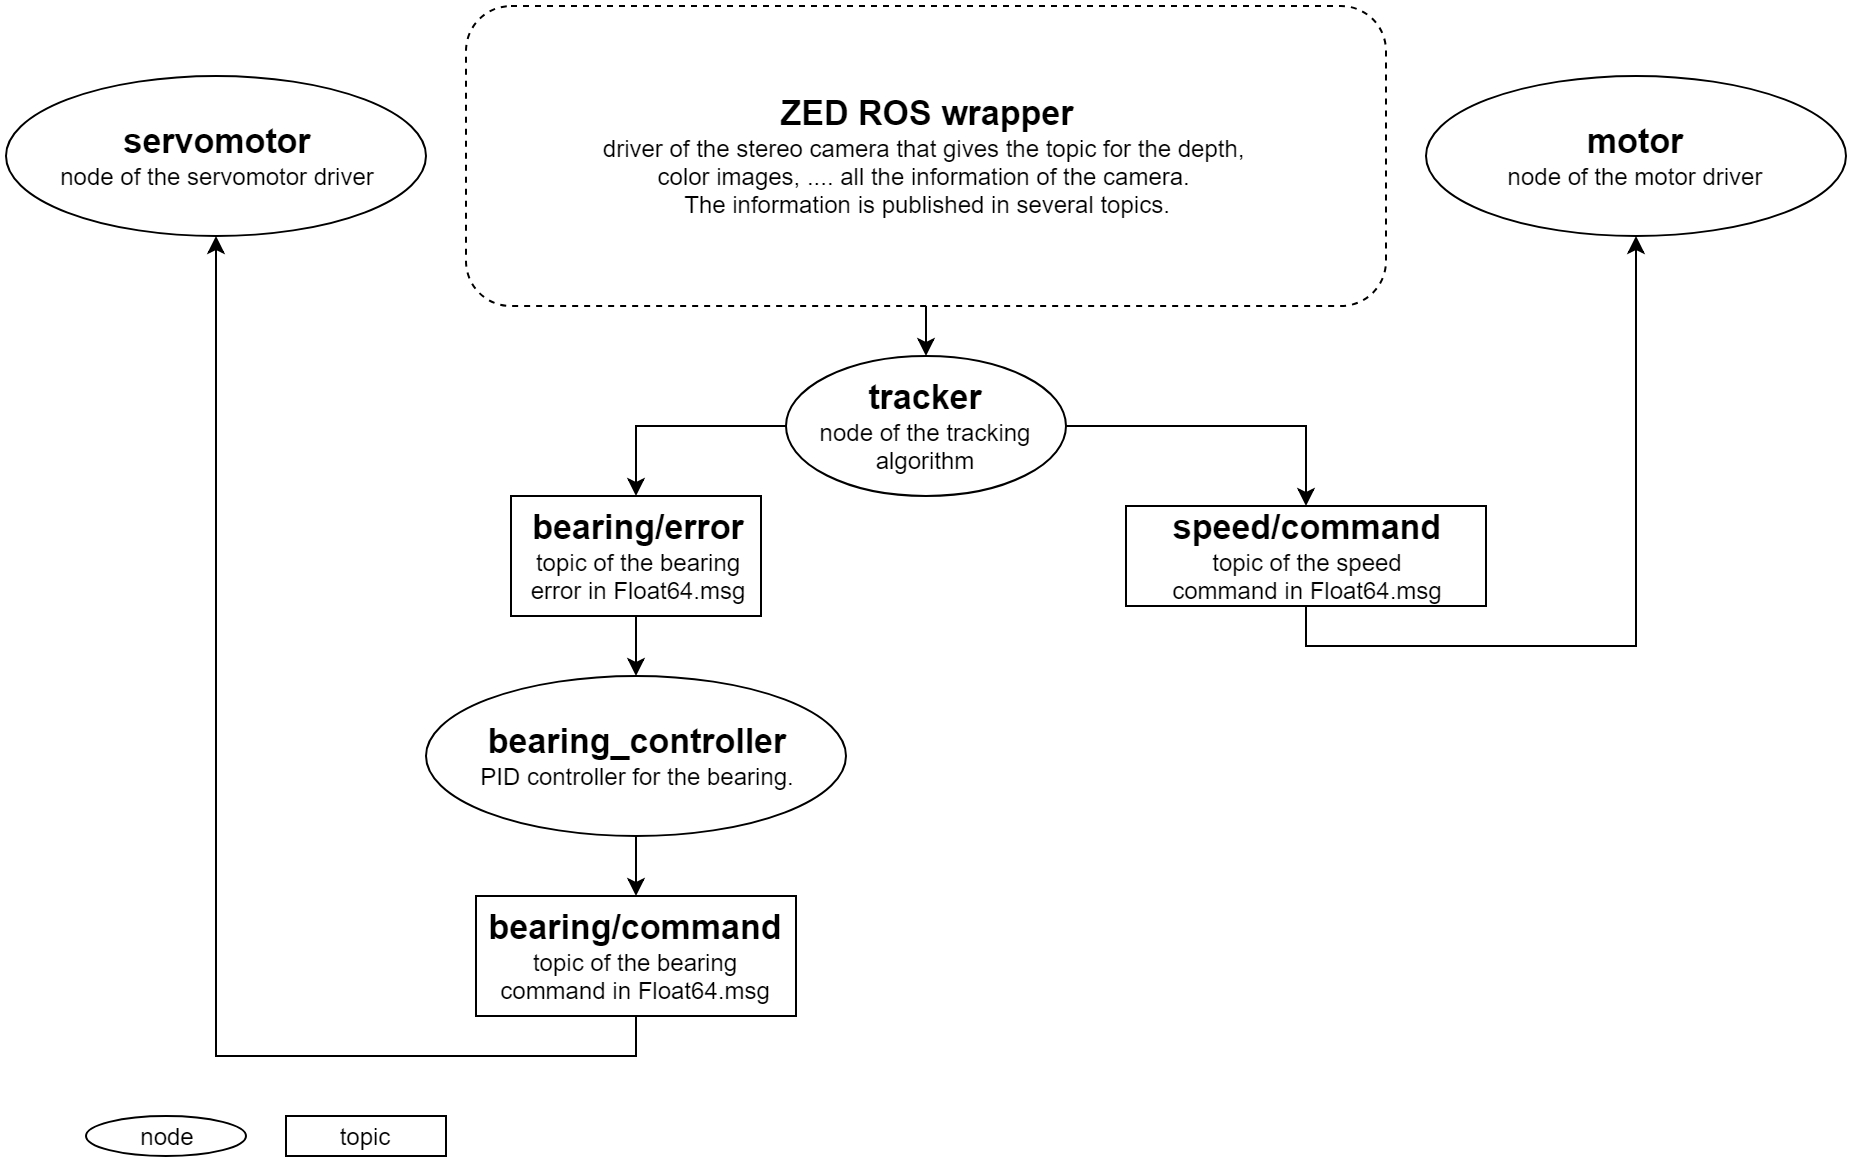
\includegraphics[width=1.0\columnwidth, height = 0.7\columnwidth]{imgs/ros.png}
			\caption{\textit{ROS} architecture.}
			\label{rosarchitecture}
		\end{figure}
		
		\FloatBarrier
		
		One way the \textit{ROS} architecture figure 
		\vref{rosarchitecture} was tested
		was to run only the nodes of the drivers on
		the \textit{Jetson Nano} since each driver needs
		to run on the hardware, which enables to do 
		any other processing on a remote computer
		for more computer power. The alternative is to run 
		all the nodes presented on figure 
		\vref{rosarchitecture} on the \textit{Jetson Nano} and 
		use a remote computer only for
		introspection purpose.
		
		\subsection{Bearing regulation}
			
		To control the bearing of the robot the \textit{RGB} images 
		of the camera are used. The \textit{GOTURN} algorithm 
		processes an image and outputs the location of the 
		target in the image by computing a bounding box. An
		error is then calculated by comparing the bounding box
		to the entire image. This error  has the following expression:
		\begin{equation}
			e = \frac{m - m_{bb}}{X}
		\end{equation}
		where $m$ is the middle of the image regarding the horizontal 
		axis or the $x$-axis. $m_{bb}$ is the middle of the bounding
		box along the horizontal axis in the frame of 
		the image. $X$ is the width of the image, which is used
		as a normalization. A \textit{PID}, or \textit{proportional
		integrate derivative} controller will tend
		to horizontally center the bounding box in the image, which 
		will entail that the robot will be directed toward 
		the target.
		% TODO in the ROS architecture
		
		\subsection{Speed regulation}
		
		In order to regulate the speed of the robot, the depth 
		information of the stereo camera is processed. Once the 
		bounding box is computed by the tracker, only 
		the depth in the area of the bounding box is considered.
		The idea is then to regulate the speed regarding the object
		in the bounding box, which is the closest to the robot.
		Neither an error needs to be computed, nor a \textit{PID}
		controller 
		needs to be implemented. The command is
		directly the depth.
		\\\indent In practice, the command is not only the raw depth.
		The matrix of the depth in the bounding box, represented 
		as $D_{bb}$ in \eqref{eq:math}, is filtered
		by a function or kernel \textit{f} which takes the median 
		of the $N$ lowest depth values in $D_{bb}$. Through that 
		process the noise in the image is filtered and
		an equivalent depth value is computed for the closest
		obstacle inside the bouding box.
		The command implementing the dynamic following of the target
		for the \textit{ESC} is as follows:
		
		\begin{comment}
		\[ \begin{cases}
			u_1 = \frac{\min\limits_{i,j \in\ bounding\ box }(d_{i,j})}{d_{max}} \times K  + \bar{u_1},,\\
			u_{1,min},\ if\ d_{i,j} \leq d_{min},\\
			u_{1,max},\ if\ d_{i,j} \geq d_{max}		
		\end{cases} \]
		\end{comment}
		
		\begin{equation}\label{eq:math}
		\begin{cases}
		u_1 = f(D_{bb})\times K + \bar{u_1},\\
		u_{1,min},\ if\ f(D_{bb}) \leq d_{min},\\
		u_{1,max},\ if\ f(D_{bb}) \geq d_{max}		
		\end{cases}
		\end{equation}
				
		The speed will gradually increase if the target rolls away.
		If the target is too far, the speed will saturate, and reversely, 
		if the target is too close, the robot will stop. 
		The parameters in the command law had to be determined
		experimentally.
		\\\indent In case a potentially dangerous obstacle is not comprised in the 
		bounding box, the tracker won't see it with the previous technique. Thus, a lidar sensor
		could be added on the front of the robot to detect obstacle in case of emergency.
		Alternatively, the entire depth matrix could be filtered and processed to detect
		other obstacles outside the bounding box and stop the robot if needed.
		
		\subsection{Unit Tests}\label{hardwaretests}
		
		In order to test the \textit{ROS} architecture, 
		for the local part, without \textit{Wifi} communication,
		everything was launched on a personal computer, \textit{Asus G703VI}.
		The stereo camera was simulated, and the commands were not 
		applied. The tests showed that the architecture
		worked as expected with a processing rate of 30 \textit{FPS},
		which far more than acceptable. The next step was the integration discussed
		in the part \vref{results}.
			
\chapter{Integration}\label{results}
	
	\introductionLettrine{T}{his} part gives an analysis of the latest results
	obtained in this project. Basically, the part tackles
	the integration of the software in the hardware. The technique 
	applied was to gradually remove each aspect of the simulation 
	environment, adding more and more real constraints at each stride.
	
	\begin{comment}
	
		> Integration of the zed camera in the ROS architecture + powered via the wall plug + wifi.
			5 FPS
		
		> With the wifi stick + in real conditions : shutdown --> power and driver problem.
		
		> Ethernet cable : Results of the integration of the hardware with the software:
		test with the remote architecture and the Ethernet cable
			5 FPS in average
			curve of the error
			several pictures showing that the robot follows the target
			
		> Test with the new wifi stick + the processing on the robot.
	
	\end{comment}
	
	\section{Integration of the ZED camera and the \textit{Wifi} communication in the ROS architecture}\label{test1}
		
		\subsection{Conditions}
		
		The goal of this integration test was to determine whether, while plugged 
		to the wall-plug, that is to say without any power-bank or 
		batterie, the tracking system was functioning correctly
		with a remote processing via \textit{Wifi}.
		\\\indent The computer \textit{Asus G703VI} was used
		as a remote computer and the \textit{Jetson Nano} was 
		used for the embedded computer on the robot. The
		actuators had not been integrated yet. Besides,\\
		\textit{the ZED camera} was used to 
		test whether the tracking process was working 
		with a real stereo camera.
		
		\subsection{Analysis}
		
		The tracking rate obtained was about 5-6 \textit{FPS} with 
		a low resolution \textit{VGA} and 4 \textit{FPS} with a \textit{720p} quality.
		The discrepancy between the 30 \textit{FPS} obtained
		in simulation, as discussed in \vref{hardwaretests}, and the 
		tracking rate in this test could be surprising at first.
		Yet, it is totally understandable considering that the 
		frames of the \textit{ZED camera} are compressed, and then sent
		to the remote computer where they are processed for tracking 
		purpose, and finally the commands are sent to the robot. 
		The commands were not applied to the hardware though.
		\\\indent Such a frame rate for the overhaul processing 
		is though acceptable, and the latencies are not 
		perceivable. The performances could be enhanced if the 
		processing was done just on the \textit{Jetson Nano}.
		It would however be more complicated to run very 
		greedy deep learning models.

	\section{Integration of the remote control}
	
		\subsection{Conditions}
		
		After having tested that the \textit{ROS} architecture
		was functioning with a real stereo camera and through 
		\textit{Wifi} communication,  the next step was to test
		whether the use of batteries was not undermining the 
		process thanks to power issues. Several batteries 
		were added : one for the motor, \textit{Li-Po 3s}, and 
		one for the embedded computer and the servomotor, however 
		not the one ordered which had not arrived yet. 
	
		\subsection{Analysis}
		
		The network established between 
		the remote station and the robot were breaking down frequently.
		It appeared that the \textit{Wifi stick} used, the
		\href{https://www.miniinthebox.com/en/p/5ghz-usb-wifi-adapter-600mbps-wifi-antenna-2dbi-support-windows-mac-802-11ac-usb-network-card-wifi-dongle-for-desktop-laptop-pc\_p5957285.html?prm=2.3.5.1}{\textit{usb wifi dongle EP-AC1607}}, since the 
		ordered one had not been delivered at that time, had 
		faulty drivers, which backfired when the \textit{Jetson Nano} was
		underpowered.
		\\\indent The test demonstrated that powering the 
		\textit{Jetson Nano} through micro-usb was not 
		sufficient. The ordered battery \textit{Krisdonia 25000mAh}
		should fix the issue.
		
	\section{Integration of the actuators}
		
		\subsection{Conditions}
		
		The goal of this test was to add the actuators 
		to the \textit{ROS} architecture and finally 
		see the robot move. To avoid the network shutdowns 
		experienced in the latter test, the communication
		between the two computers
		was handled via \textit{Ethernet}, and the batteries
		were used. 
		
		\subsection{Analysis}
		
		No network shutdowns were experienced, and 
		the tracking rate was identical to
		the results obtained in the test 
		presented in \vref{test1}. The test 
		showed that the \textit{Wifi stick}
		had in fact a faulty driver, and that 
		power was also an issue to solve.
		The components of the hardware architecture in \vref{hardwareoverview} were chosen
		to meet these requirements.
		
\chapter{Setup}\label{setup}

	\introductionLettrine{T}{his} part presents the material needed and the 
	necessary conditions to replicate the \hyperref[results]{results}\footnote{cf. \vref{results}.} of
	this project. Should you need some explanations on the project, please
	refer to parts \vref{context}, \vref{stateofart}, \vref{hardware}, and \vref{software}.

	\section{Hardware setup}

	% TODO
	% wiring, blueprint of the wiring (or maybe use the same than the hardware architecture)
	
	\begin{itemize}
		\item [\ding{55}] \underline{Computers} : Jetson Nano, Ubuntu 18.04, remote computer Ubuntu 18.04. 
	\end{itemize}
	
	
	\section{Software setup}